\documentclass[
  11pt,
  letterpaper,
   addpoints,
   answers
  ]{exam}

\usepackage{../exercise-preamble}
\usepackage{float}
\begin{document}

\noindent
\begin{minipage}{0.47\textwidth}

\includegraphics[width=\textwidth]{../fcfm_die}
\end{minipage}
\begin{minipage}{0.53\textwidth}
\begin{center} 
\large\textbf{Conversión de la Energía y Sistemas Eléctricos } (EL4111-1) \\
\large\textbf{Clase auxiliar Extra} \\
\small Prof.~Constanza Ahumada - Rodrigo Moreno.\\
\small Prof.~Aux.~Javiera Pacheco - Erik Sáez\\
\small Ayudantes.~Manuel Aceituno - Pamela Acuña - Alvaro Flores\\
\end{center}
\end{minipage}

\vspace{0.5cm}
\noindent
\vspace{.85cm}

\begin{questions}
    %%%%%%%%%%%%%%%%%%%%%%%%%%%
    \question El generador síncrono de una central termoeléctrica de ciclo combinado venía con la carta de operación que se muestra en la figura, la cual fue provista por el fabricante y en donde se puede apreciar que el eje horizontal corresponde a la potencia reactiva, en [MVAr], y el vertical a la potencia activa, en [MW].

    \begin{figure}[h!]
        \centering
        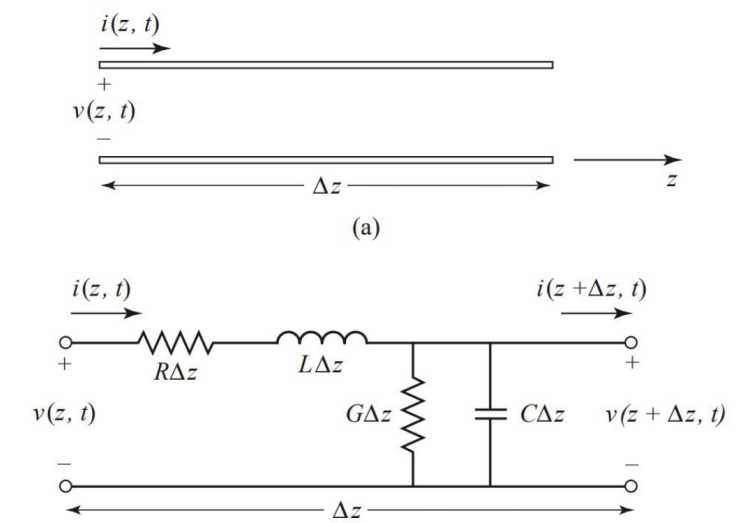
\includegraphics[width=0.5\textwidth]{Auxiliar_7_1} % Cambia "ruta_de_la_imagen" por la ubicación de tu archivo
        \caption{Carta de operación del generador síncrono.}
    \end{figure}
    Esta máquina es de tensión nominal 23 [kV], la tensión interna máxima y mínima es de 2.5 y 0.5 veces la nominal respectivamente. Por otro lado, la reactancia síncrona es de 3.6 [\(\Omega\)] y el límite de estabilidad está fijado en $70^{\circ}$. A través de su largo periodo en funcionamiento, la máquina ha tenido algunos incidentes y desgastes, los cuales han modificado los valores anteriores. Entre ellos se encuentran:
    \begin{itemize}
        \item La ruptura y posterior extracción de una turbina de gas de la máquina motriz, lo que redujo en 20\% la potencia activa máxima que esta podía entregar al generador.
        \item La quema del 15\% de los devanados del estator.
        \item La quema del 10\% del devanado del circuito de campo.
    \end{itemize}
    A partir de lo anteriormente mencionado, determine los nuevos límites de la carta de operación describiéndolos claramente mediante ecuaciones de la forma \( P(Q) \). Para ello, asuma que existe una relación directamente proporcional entre el número de vueltas del devanado de campo y la tensión interna.
    
    
    
    %%%%%%%%%%%%%%%%%%%%%%%%%%%
    \begin{solution}
        \subsection*{Resolucion 1.1}
        Debemos recordar que los factores que limitan la carta de operacion son:
        \begin{itemize}
            \item \textbf{Maxima y minima potencia activa}: En un generador, el límite de operación para la potencia activa \( P \) es \( P \geq 0 \) y está limitado en el eje de la potencia reactiva \( Q \). En generadores térmicos de rotor cilíndrico, existe un límite mínimo \( P_{\text{min}} \), generalmente alrededor del 30\% de la potencia nominal, para asegurar el manejo adecuado del fuego. Además, la turbina puede imponer un límite máximo \( P_{\text{max}} \) en la potencia activa debido a sus propias restricciones. Aunque en una central bien planificada el generador debería ajustarse a la potencia de la turbina, en algunos casos el límite \( P_{\text{max}} \) puede quedar fuera del rango del generador debido a variaciones en el mercado de generadores. Estas se visualizan como lineas constantes.

            \item \textbf{Maxima corriente de armadura:} En las máquinas reales, la corriente de armadura tiene un valor máximo impuesto por el calentamiento del estator y la vida útil del aislamiento. Este límite establece una circunferencia en la carta de operación con centro en el origen y radio \( V_{\text{imax}} \). Por razones económicas, se opera con una combinación de \( P \) y \( Q \), por lo que este límite es ligeramente superior al de la máxima potencia activa, es decir, \( V_{\text{imax}} \geq P_{\text{max}} \). En la intersección de ambos límites se alcanza el factor de potencia nominal. Este límite puede sobrepasarse brevemente, ya que se relaciona con el calentamiento acumulado.

            \item \textbf{Maxima y minima corriente de excitacion:} Dado que existe un valor máximo para la corriente de excitación, impuesto por el calentamiento del rotor o las características de la excitatriz, se genera un límite para la operación del generador, representado por una circunferencia de centro \( \left(-\frac{V^2}{x_s}, 0\right) \) y radio \( \frac{V_{\text{Emax}}}{x_s} \). Este límite es generalmente inferior al de la corriente de armadura, afectando principalmente a cargas inductivas pequeñas. Por otro lado, en la práctica, no es posible alcanzar la mínima excitación teórica (\( E = 0 \)) debido a flujos residuales de la excitatriz. En general, se estima una excitación mínima \( E_{\text{min}} \) entre 5\% y 10\% de la necesaria con carga nominal, generando así un límite de operación con centro \( \left(-\frac{V^2}{x_s}, 0\right) \) y radio \( \frac{V_{\text{Emin}}}{x_s} \). Esto limita la potencia reactiva absorbida por el generador.

            \item \textbf{Limite de estabilidad permanente}: Existe una limitación de operación en una máquina síncrona impuesta por la inestabilidad que ocurre al alcanzar un ángulo de carga \( \delta = 90^\circ \) en máquinas de rotor cilíndrico. Este límite teórico se representa como una recta paralela al eje \( P \) que pasa por el punto \( \left(-\frac{V^2}{x_s}, 0\right) \), donde la potencia reactiva \( Q \) es negativa. Debido a que trabajar en este límite es poco aconsejable por la dificultad en controlar variaciones de carga, se define un \textbf{límite práctico de estabilidad}, generalmente basado en experiencias de operación. Este límite práctico se representa como una recta que parte del punto \( \left(-\frac{V^2}{x_s}, 0\right) \) y forma un ángulo de 70° con respecto al eje de la potencia reactiva \( Q \).
        \end{itemize}
        Tomando en consideracion todo lo anterior podemos comenzar a considerar aspectos visuales en la carta de operacion entregada para poder determinar los nuevos limites de operacion, por ejemplo:
        \begin{align}
            P_{max} &= 60[MW]\\
            P_{min} &= 20[MW]\\
            S_{max} &= V \cdot I_{max}= 80[MVA]
        \end{align}
        Este ultimo se puede obtener dado que corresponde a la semi circunferencia centrada en 0 y con radio $V \cdot I_{max}$. Luego debemos considerar el voltaje nominal:
        \begin{align}
            V_{nom} = \frac{23[kVff]}{\sqrt{3} = 13.2791[kVfn]}
        \end{align}
        Luego de los incidentes mencionados se deberan tener las siguientes consideracion para los nuevos valores:
        \begin{itemize}
            \item Ruptura y posterior extracción de una turbina
            \begin{align}
            P'_{\text{max}} &= 0.8 \cdot P_{\text{max}} = 48 \, \text{MW}
            \end{align}
        
            \item La quema del 15\% de los devanados del estator
            \begin{align}
            X'_{s} &= 0.85 \cdot X_{s} = 3.06 \, \Omega
            \end{align}
        
            \item La quema del 10\% de los devanados del circuito de campo
            \begin{align}
            E'_{\text{max}} &= 0.9 \cdot E_{\text{max}} = 0.9 \cdot 2.5 \cdot V_{\text{nom}} = 29.8778 \, \text{kV} \\
            E'_{\text{min}} &= 0.9 \cdot E_{\text{min}} = 0.9 \cdot 0.5 \cdot V_{\text{nom}} = 5.9755 \, \text{kV}
            \end{align}
        \end{itemize}
        
        Con lo anterior es posible calcular las nuevas curvas de la carta de operación.
        
        \begin{enumerate}
            \item \textbf{Máxima potencia activa}
            \begin{align}
            P'_{\text{max}} &= 48 \, \text{MW} \\
            P(Q) &= 48
            \end{align}
        
            \item \textbf{Mínima potencia activa}
            \begin{align}
            P_{\text{min}} &= 20 \, \text{MW} \\
            P(Q) &= 20
            \end{align}
        
            \item \textbf{Máxima corriente de armadura}
            \begin{align}
            S_{\text{max}} &= V_{\text{nom}} \cdot I_{\text{max}} = 80 \, \text{MVA} \\
            P(Q) &= \sqrt{80^2 - Q^2}
            \end{align}
        
            \item \textbf{Máxima excitación}
            \begin{itemize}
                \item Centro:
                \begin{align}
                \left( \frac{V_{\text{nom}}^2}{X'_s}, 0 \right) &= (-57.6252, 0)
                \end{align}
                
                \item Radio:
                \begin{align}
                \frac{V_{\text{nom}} \cdot E'_{\text{max}}}{X'_s} &= 129.6568 \\
                \Rightarrow P(Q) &= \sqrt{129.6568^2 - (Q + 57.6252)^2}
                \end{align}
            \end{itemize}
        
            \item \textbf{Mínima excitación}
            \begin{itemize}
                \item Centro:
                \begin{align}
                \left( \frac{V_{\text{nom}}^2}{X'_s}, 0 \right) &= (-57.6252, 0)
                \end{align}
        
                \item Radio:
                \begin{align}
                \frac{V_{\text{nom}} \cdot E'_{\text{min}}}{X'_s} &= 25.9313 \\
                \Rightarrow P(Q) &= \sqrt{25.9313^2 - (Q + 57.6252)^2}
                \end{align}
            \end{itemize}
        
            \item \textbf{Límite de estabilidad}
            \begin{itemize}
                \item Recta:
                \begin{align}
                P &= m \cdot Q + n
                \end{align}
                
                donde
                \begin{align}
                m &= \tan(70^\circ) = 2.7474
                \end{align}
        
                \item Al evaluar la recta anterior en el punto \( \left( -\frac{V_{\text{nom}}^2}{X'_s}, 0 \right) = (-57.6252, 0) \), se tendrá que:
                \begin{align}
                0 &= 2.7474 \cdot (-57.6252) + n \\
                n &= 158.3196
                \end{align}
                
                \begin{align}
                \Rightarrow P(Q) &= 2.7474 \cdot Q + 158.3196
                \end{align}
            \end{itemize}
        \end{enumerate}
        
        En la siguiente figura se muestra la nueva carta de operación obtenida a partir de las curvas anteriores.
        \begin{center}
            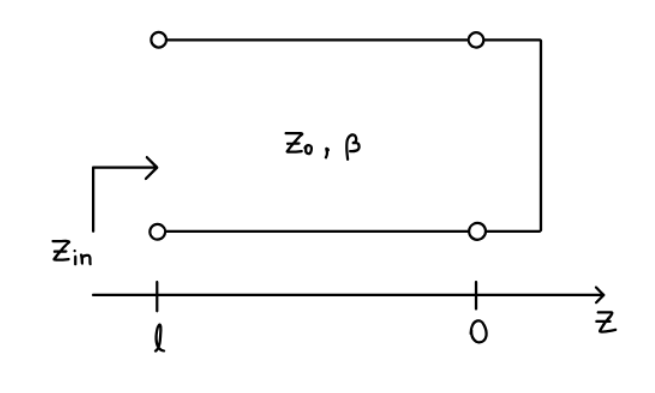
\includegraphics[width=0.7\textwidth]{Auxiliar_7_2} \\
            \textit{Carta de operacion posterior a las modificaciones.}
        \end{center}
    \end{solution}
    %%%%%%%%%%%%%%%%%%%%%%%%%%%
    \question Un generador síncrono trifásico de 50 [MVA], 13,8 [kV], 4 polos y 50 [Hz] presenta los siguientes datos de corriente de campo \( I_f \) y tensión interna \( E \) en su prueba de vacío:

    \begin{table}[h!]
        \centering
        \caption{Resultados de prueba de circuito abierto.}
        \begin{tabular}{|c|c|c|c|c|c|c|}
            \hline
            Excitación \( I_{fd} \) [A] & 61 & 92 & 142 & 179 & 200 & 240 \\
            \hline
            Prueba de CA \( E \) [$V_{ff}$] & 5520 & 8325 & 11040 & 12420 & 13100 & 14395 \\
            \hline
        \end{tabular}
    \end{table}
    
    Además, para el ensayo de cortocircuito se necesitaron 242 [A] de corriente de excitación para lograr una corriente de 2090 [A].
    
    \begin{enumerate}
        \item[a)] Determine la reactancia saturada y no saturada de la máquina.
    
        \item[b)] Si en cierto instante en que la máquina se encuentra operando como generador conectada a una barra infinita de igual frecuencia y tensión nominal, inyecta 36 [MW] con factor de potencia 0,85 inductivo. Determine la corriente y la tensión interna (magnitud y ángulo) de la máquina en este punto de operación. Bosqueje el circuito que representa esta situación y el respectivo diagrama fasorial. Indique también si el generador está operando subexcitado o sobreexcitado.
    
        \item[c)] Suponga que debido a un cambio constructivo en la máquina, la reactancia síncrona pasa a ser \( x_s = 5 \, [\Omega] \). Dibuje la carta de operación de la máquina indicando todos sus límites y a qué se deben estos límites si: \( P_{\text{max}} = 40 \, [\text{MW}] \), \( P_{\text{min}} = 5 \, [\text{MW}] \), \( E_{\text{min}} = 4 \, [\text{kV}] \), \( E_{\text{max}} = 36 \, [\text{kV}] \) y el ángulo del límite de estabilidad de la máquina es de 75°. Además, calcule e indique en la carta de operación el factor de potencia nominal y la corriente máxima por el estator.
    \end{enumerate}
%%%%%%%%%%%%%%%%%%%%%%%%%%%
\begin{solution}
El desarrollo de el item a y b, son los ya visto en el auxiliar 6, por lo que nos centraremos en obtener la carta de operacion bajo esas condiciones:
\subsection*{Resolucion 2.3}
Dado que nos interesa el obtener la carta de operacion de la maquina, debemos obtener los limites de operacion de la maquina por lo tanto:
\begin{itemize}
    \item Tenemos que los limites asociados a las potencias vienen dados de manera directa por $P_{max} = 40[MW]$ y $P_{min} = 5[MW]$.
\end{itemize}
Luego para obtener la corriente maxima por el estator, debemos considerar que el voltaje 13.8[kV] corresponde a un voltaje de linea, por lo tanto tenemos la siguiente relacion para los valores nominales(\textit{Si no recuerda las relaciones le puede ser util el siguiente video \href{https://www.youtube.com/watch?v=8dIj_e6PR-k}{link}
}):
\begin{align}
    S_{max} &= \sqrt{3} \cdot V_{ff} \cdot  I_{ff}\\
    I_{ff} &= \frac{S_{max}}{\sqrt{3} \cdot V_{ff}} = \frac{50[MVA]}{\sqrt{3} \cdot 13.8[kV]} = 2.0875[kA]
\end{align}
Luego recordando las relacion trigonometrica que asocia la potencia activa con la potencia aparente y el factor de potencia, se tiene que:
\begin{align}
    \frac{P_{3\phi}}{S_{3\phi}}= \frac{40 [MW]}{MVA} = 0.8 = FP
\end{align}
De esta manera se obtiene el valor del factor de potencia. Luego es de interes conocer el centro de la circunfernecia asociada a las corriente de maxima y minima excitacion, por lo tanto se tiene que:
\begin{align}
    \left( -\frac{V^2}{x_s}, 0 \right) = \left( -\frac{13.8^2}{5}, 0 \right) = (-38.088[M] , 0)
\end{align}
Con esto podemos obtener los radios minima y maximo tales que:
\begin{align}
    \text{Radio minimo:} & \frac{V_{ff} \cdot E_{min}}{X_{s}} = 11.7[M] \\
    \text{Radio maximo:} & \frac{V_{ff} \cdot E_{max}}{X_{s}} = 99.36[M]
\end{align}
Un importante aspecto a considerar esque tambien es posible trabar con el $V_{fn}$ realizando la respectiva conversion. Por ultimo para la estabilidad tenemos que corersponde a una pendiente de 75° que cruza el punto $\left( \frac{-v^{2}}{x_{s}},0\right)$. Teniendo en consideracion todo lo anterior se concluye que 
\begin{center}
    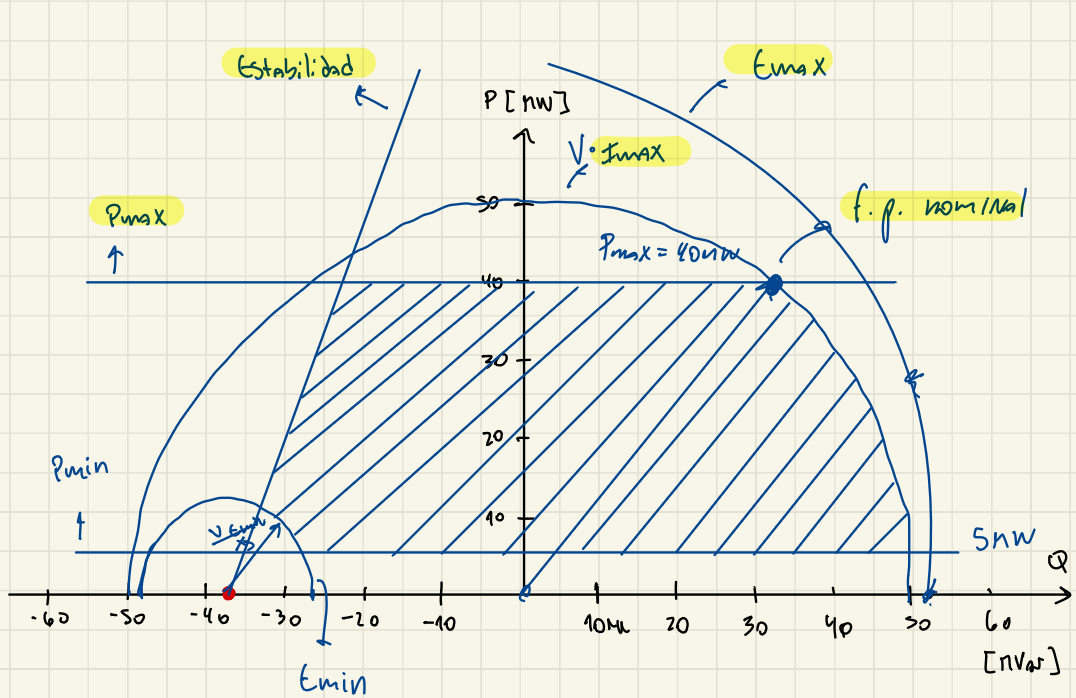
\includegraphics[width=0.8\textwidth]{Resumen_23} \\
\end{center}
Notemos que todo el desarrollo se realizo para una configuracion trifasica , para la monofasica tienen el ejemplo anterior.
 \end{solution}
%%%%%%%%%%%%%%%%%%%%%%%%%%%
\question Se tienen 2 motores shunt de corriente continua. Ambos motores operan con voltaje nominal de 220 V, girando a 1000 RPM y absorbiendo 20 kW cada uno a plena carga. Mediante las pruebas respectivas se sabe que:

\begin{table}[H]
    \centering
    \begin{tabular}{|c|c|c|}
        \hline
        Motor & $R_a \, [\Omega]$ & $R_c \, [\Omega]$ \\
        \hline
        I & 0.1 & 38 \\
        II & 0.08 & 40 \\
        \hline
    \end{tabular}
\end{table}

Suponga que se conectan ambos motores en paralelo, acoplados por el mismo eje y se operan como generadores para alimentar la calefacción de una empresa. Dicha calefacción está compuesta exclusivamente por elementos pasivos y tiene un leve carácter inductivo. Bajo condiciones nominales, es decir, $220 \, V \, AC$, absorbe $35 \, kW$ con un $\cos(\phi) = 0.9$. Desprecie las pérdidas mecánicas.

\begin{enumerate}
    \item[a)] Calcular el torque necesario sobre el eje para que la calefacción entregue la misma potencia que en condiciones nominales.
    \item[b)] La potencia eléctrica entregada al eje.
\end{enumerate}
%%%%%%%%%%%%%%%%%%%%%%%%%%%
\begin{solution}
   \subsection*{Resolucion 3.1}
   Se busca obtener el torque necesario para que la calefaccion entregue la misma potencia que en condiciones nominales, por lo que primero se obtendra la frecuencia de operacion:
   \begin{align}
    n&= 1000 [rpm]\\
    w&= \frac{2\pi \cdot n}{60} = 104.72 [rad/s]
   \end{align}
   Luego considerando los motores por separados tenemos que los torques seran:
   \subsubsection*{Para el motor 1}
   En condiciones nominales se tendra que el motor absorve 20[kW] para los 220[V], por tanto:
   \begin{align}
        I_{l} = \frac{P_{nominal}}{V_{nominal}} = \frac{20[kW]}{220[V]} = 90.91[A]
   \end{align}
   Luego la corriente de campo considerando la resistencia, tenemos que:
   \begin{align}
        I_{c} = \frac{220[V]}{38[\Omega]} = 5.79[A]
   \end{align}
   Con esto, es posible obtener la corriente de armadura como:
   \begin{align}
        I_{a} = i_{l} - i_{c} = 85.12[A] 
   \end{align}
   De esta manera tenemos que:
   \begin{align}
        V_{a} &= E_{a} + I_{a} \cdot R_{a}\\
        E_{a} &= V_{a} - I_{a} \cdot R_{a} = 220[V] - 85.12[A] \cdot 0.1[\Omega] = 211.49[V] 
   \end{align}
   De esta manera se obtiene que el torque vendra dado por:
   \begin{align}
       G_{1}= \frac{E_{a}}{\omega i_{c} } =0.3488 
   \end{align}
   Luego de manera analogamente para el otro motor:
   \subsubsection*{Para el motor 2}
   Tenemos que:
   \begin{align}
        I_{l} = \frac{P_{nominal}}{V_{nominal}} = \frac{20[kW]}{220[V]} = 90.91[A]
   \end{align}
   Luego la corriente de campo vendra dada por:
    \begin{align}
          I_{c} = \frac{220[V]}{40[\Omega]} = 5.5[A]
    \end{align}
    De esta manera tenemos que la corriente de armadura para el motor 2 es:
    \begin{align}
        I_{a} = i_{l} - i_{c} = 85.41[A]
    \end{align}
    Luego tenemos que la tensión en el inducido es:
    \begin{align}
        V_{a} &= E_{a} + I_{a} \cdot R_{a}\\
        E_{a} &= V_{a} - I_{a} \cdot R_{a} = 220[V] - 85.41[A] \cdot 0.08[\Omega] = 213.39[V]
    \end{align}
    Con lo que $G_{2}$ se tendra que:
    \begin{align}
        G_{2}= \frac{E_{a}}{\omega i_{c} } =0.3886
    \end{align}
    Una vez obtenido los valores de G, se que para obtener el valor de $i_{e}$ (\textit{asociado a la estufa}), tenemos que considerar el efecto de la estufa, por tanto:
    \begin{align}
        S_{e}\cos(\phi) &= P_{e}\\
        S_{e} &= \frac{P_{e}}{\cos(\phi)} = \frac{35[kW]}{0.9} = 38.89[kVA]
    \end{align}
    Considerando que la potencia activa viene dada por:
    \begin{align}
        P_{e} = R_{e} \cdot \|i_{e}\|^2
    \end{align}
    por otro lado tenemos que:
    \begin{align}
        \|I_{e}\| & = \frac{\|S_{e}\|}{V_{nominal}}
    \end{align}
    Luego se puede obtener que:
    \begin{align}
        R_{e} &= \frac{P_{e} \cdot \|V_{nom}\|^{2}}{\|S_{e}\|^{2}} = \frac{35[kW] \cdot 220[V]^{2}}{38.89[kVA]^{2}} = 1.1201[\Omega]
    \end{align}
    Luego podemos hacer un modelo circuital para entender el sistema y como se mueven las corrientes, por tanto:
    \begin{center}
        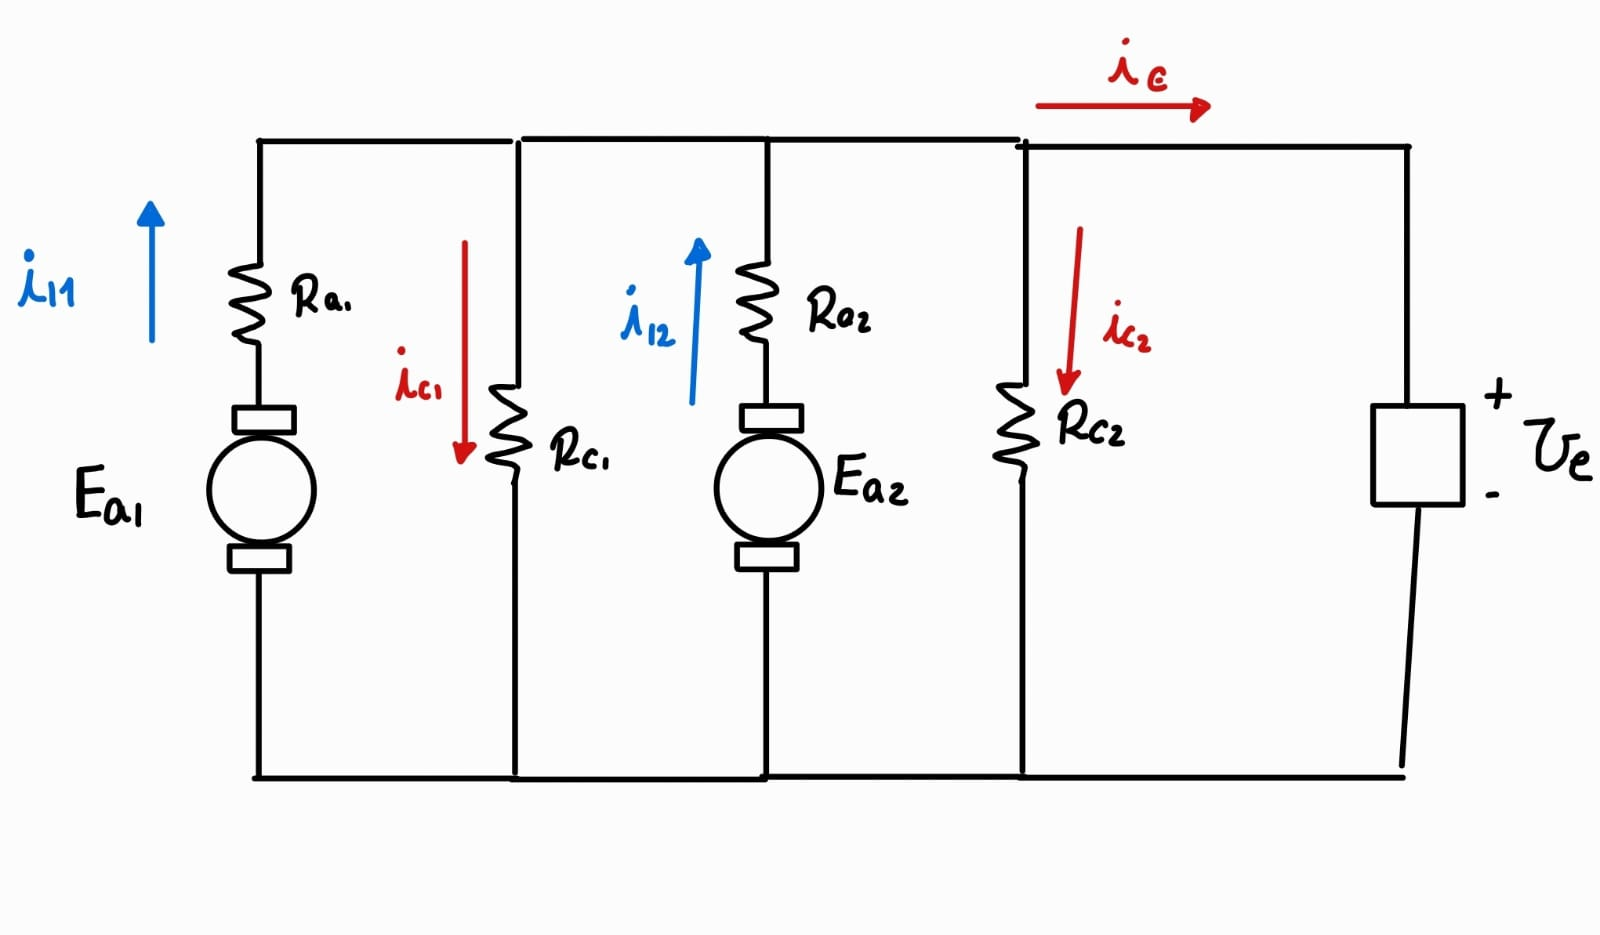
\includegraphics[width=0.6\textwidth]{Auxiliar_7_3} \\
    \end{center}
    Luego tenemos que la corriente $i_{e}$ viene dado por:
    \begin{align}
        P_{e} = R_{e} \cdot \|i_{e}\|^{2} \Rightarrow \|i_{e}\| = \sqrt{\frac{P_{e}}{R_{e}}} = 176.7688[A]
    \end{align}
    El voltaje de la estufa sera:
    \begin{align}
        V_{e}= \frac{35[kW]}{176.7688[A]} = 197.99[V]
    \end{align}
    De esta manera al estar en paralelo los circuitos podemos obtener las corrientes de campo para ambos motores como:
    \begin{align}
        i_{c1}&= \frac{V_{e}}{R_{c1}}= 5.21[A]\\
        i_{c2} = \frac{V_{e}}{R_{c2}}= 4.95[A]
    \end{align}
    Luego tenemos que haciendo ley de kirchoff en los diferentes nodos, se logra obtener que:
    \begin{align}
        i_{l1} + i_{l2} = i_{c1} + i_{c2} + i_{e} 
    \end{align}
    Donde las primeras corresponden a las corrientes salientes del motor y las segundas a las corrientes consumidas. De esta manera se tiene que considerando la \textbf{operacion como generador:}
    \begin{align}
        V_{e} &= E_{a1} - i_{l1} \cdot R_{a}\\
        i_{l1} &= \frac{E_{a1}- V_{e}}{R_{a1}}
    \end{align}
    Analogamente tenemos que para el otro generador
    \begin{align}
        V_{e} &= E_{a2} - i_{l2} \cdot R_{a2}\\
        i_{l2} &= \frac{E_{a2}- V_{e}}{R_{a2}}
    \end{align}
    Ademas tenemos que los $\omega$ son iguales para ambos motores, por lo que se tiene que:
    \begin{align}
        E_{a1} &= \omega \cdot i_{c1} \cdot G_{1}\\
        E_{a2} &= \omega \cdot i_{c2} \cdot G_{2}
    \end{align}
    Donde los valores de $G_{1}$ y $G_{2}$ son los obtenidos anteriormente. Reemplazando todos los valores se llega a:
    \begin{align}
        i_{l1} + i_{l2} &= i_{c1} + i_{c2} + i_{e}\\ 
        \frac{E_{a1} - V_{e}}{R_{a1}} + \frac{E_{a2} - V_{e}}{R_{a2}} &= i_{c1} + i_{c2} + i_{e}\\
        \frac{\omega \cdot i_{c1} \cdot G_{1} - V_{e}}{R_{a1}} + \frac{\omega \cdot i_{c2} \cdot G_{2} - V_{e}}{R_{a2}} &= i_{c1} + i_{c2} + i_{e}
    \end{align}
    Con lo que todos los valores son conocidos menos $\omega$, de esta manera tenemos que despejando se llega a:
    \begin{align}
        \omega = \frac{\frac{V_{e}}{R_{a1}} + \frac{V_{e}}{R_{a2}} +i_{c1} + i_{c2} +i_{3} }{ \left( \frac{G_{1} i_{c1}}{R_{a1}} + \frac{G_{2}i_{c2}}{R_{a2}}\right)}
    \end{align}
    Reemplazando todos los valores se obtiene que $\omega = 113.0127 [rad/s]$ y por lo tanto tendremos que:
    \begin{align}
        E_{a1} & = G_{1} \cdot i_{c1} \cdot \omega = 205.39[V]\\
        E_{a2} &= G_{2} \cdot i_{c2} \cdot \omega = 207.03[V]
    \end{align}
    Con lo que se obtiene que las corrientes de armadura seran:
    \begin{align}
        I_{a1} &= \frac{E_{a1} - V_{e}}{R_{a1}} = 73.9310[A]\\
        I_{a2} &= \frac{E_{a2} - V_{e}}{R_{a2}} = 113[A]
    \end{align}
    Considerando que $V_{1} =V_{2} = V_{e}$, con lo que finalmente es posible el obtener el toruqe como:
    \begin{align}
        T_{1} &= \frac{E_{a1} \cdot I_{a1}}{\omega} = 134.3638[Nm]\\
        T_{2} &= \frac{E_{a2} \cdot I_{a2}}{\omega} = 207.03[Nm] 
    \end{align}
    Con lo que el torque total sera:
    \begin{align}
        T_{total} = T_{1} + T_{2} = 341.3938[Nm]
    \end{align}
    \subsection*{Resolucion 3.2}
    Se puede obtener la potencia electrica entregada al eje sera:
    \begin{align}
        T_{mec} &= \frac{P_{eje}}{\omega}\\
        P_{eje} &= T_{mec} \cdot \omega = 38.89[kW]
    \end{align}


\end{solution}
%%%%%%%%%%%%%%%%%%%%%%%%%%%
\question Una empresa recientemente compró una pequeña central hidroeléctrica de pasada, cuya máquina síncrona tiene una placa que indica los siguientes datos: potencia nominal $100 \, \text{MVA}$, tensión nominal $13.8 \, \text{kV}$, frecuencia $50 \, \text{Hz}$ y 24 polos. La empresa le encarga realizar las pruebas de cortocircuito y de vacío para determinar la reactancia de la máquina, arrojando los resultados de las Tablas 1 y 2.

\begin{table}[H]
    \centering
    \caption{Resultados prueba de circuito abierto.}
    \begin{tabular}{|c|c|c|c|c|c|c|c|}
        \hline
        Excitación $I_{fd}$ [A] & 50 & 100 & 200 & 300 & 400 & 600 \\
        \hline
        Prueba de CA $E$ [V$_{\text{fn}}$] & 1625 & 3250 & 6500 & 7500 & 7960 & 8800 \\
        \hline
    \end{tabular}
\end{table}

\begin{table}[H]
    \centering
    \caption{Resultados prueba de cortocircuito.}
    \begin{tabular}{|c|c|c|}
        \hline
        $I_{fd}$ [A] & 50 & 100 \\
        \hline
        $I_A$ [A] & 2050 & 4100 \\
        \hline
    \end{tabular}
\end{table}

\begin{enumerate}
    \item Determine la impedancia síncrona saturada y no saturada para la tensión nominal de la máquina.
    \item Si en cierto instante en que la máquina se encuentra operando como generador conectado a una barra infinita de igual frecuencia y tensión nominal, inyecta $72 \, \text{MW}$ con factor de potencia 0.8 inductivo. Determine la corriente, la tensión interna (magnitud y ángulo), torque y velocidad de sincronismo de la máquina en este punto de operación.
    \item Bosqueje el circuito que representa esta situación y el respectivo diagrama fasorial. Indique también si el generador está operando subexcitado o sobreexcitado.
\end{enumerate}

%----------------------------
\begin{solution}
    \subsection*{Resolucion 4.1}
    Tenemos que debemos pasar los valores  $S_{3 \phi}$ y $V_{3 \phi}$ a $S_{1 \phi}$ y $V_{1 \phi}$, por lo que se tiene que:
    \begin{align}
        S_{1 \phi} &= \frac{S_{3 \phi}}{3} = \frac{100[MVA]}{3} = 33.33[MVA]\\
        V_{1 \phi} &= \frac{V_{3 \phi}}{\sqrt{3}} = \frac{13.8[kV]}{\sqrt{3}} = 7.97[kV]
    \end{align}
    Luego queremos obtener la reactancia $Z_{sat}$ y $Z_{nsat}$, por lo que primero se obtendra la reactancia saturada recordando que:
    \begin{center}
        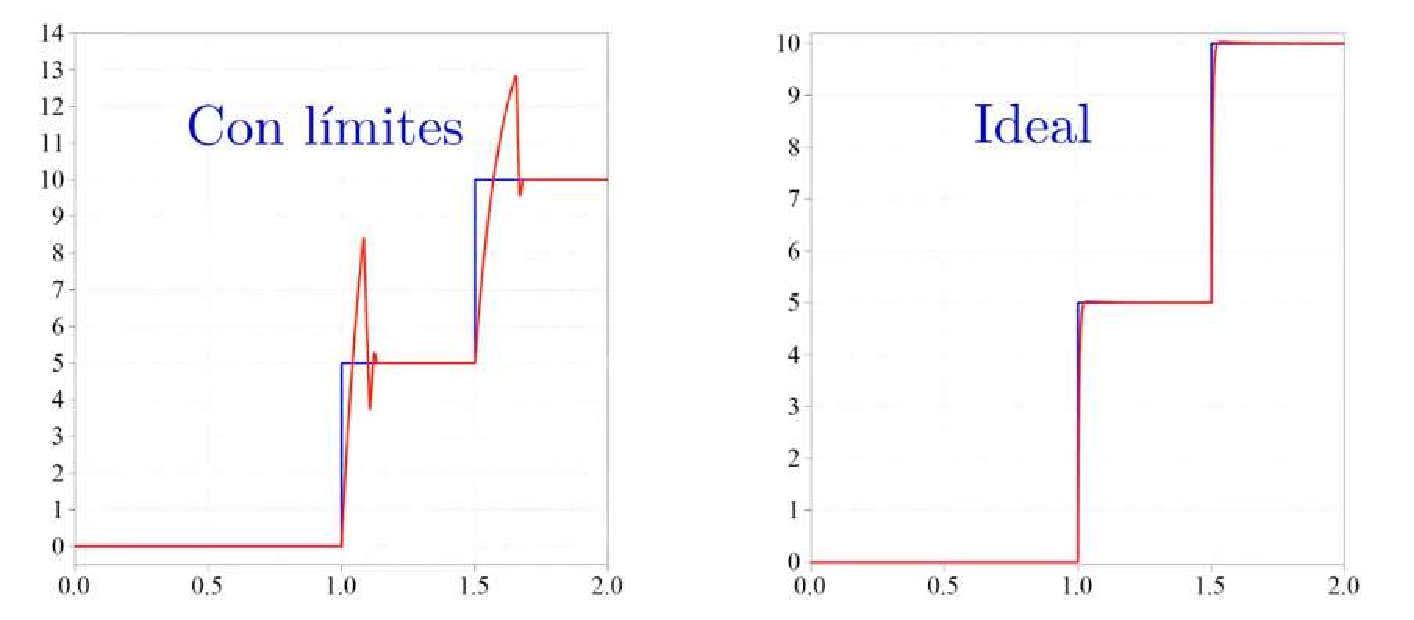
\includegraphics[width=0.4\textwidth]{Auxiliar_6_4} \\
        \textit{Curvas que permiten analizar las pruebas de cortocircuito y de vacío.}
    \end{center}
    Recordemos que las impedancias saturada y no saturada corresponden a:
    \begin{align}
        Z_{\text{sat}} &= \frac{\overline{AB}[V]}{\overline{AD}[A]}\\
        Z_{\text{nsat}} &= \frac{\overline{AC}[V]}{\overline{AD}[A]} 
    \end{align}
    Para la saturada tenemos que considerando la tension de $V_{1\phi}$ para la prueba de CA tenemos que le correspondera una corriente de campo de $I_{fd} = 400[A]$, por lo que ahora se necesita la corriente de armadura, por lo que se tiene que el comportamiento de dicha curva es lineal, es decir:
    \begin{align}
        I_{a} = m \cdot I_{f} 
    \end{align}
    y en base a los datos entregados en el enunciado para la prueba de cortocircuito se tiene de manera directa que:
    \begin{align}
        m = \frac{4100}{100} = 41
    \end{align}
    Con lo que la corriente de armadura para los 400 [A] de campo sera:
    \begin{align}
        I_{a} = 41 \cdot 400 = 16400[A]
    \end{align}
    De esta manera tenemos que la impedancia saturada sera:
    \begin{align}
        Z_{\text{sat}} = \frac{7960[V]}{16400[A]} = 0.4854[\Omega]
    \end{align}
    Por otro lado para la impedancia no saturada se tiene que podemos tomaar el punto inicial de la curva de vacio, es decir, $I_{f} = 50[A]$ y $E = 1625[V]$, por lo que se tiene que se tendra directamnete que la corriente de armadura sera:
    \begin{align}
        I_{a} = 41 \cdot 50 = 2050[A]
    \end{align}
    Esto debido a que es lineal y no satura en este caso, con lo que la corriente no saturada sera:
    \begin{align}
        Z_{\text{nsat}} = \frac{1625[V]}{2050[A]} = 0.7927[\Omega]
    \end{align}
    \subsection*{Resolucion 4.2}
    Dado que en cierto instante la maquina opera como generador conectado a una barra inifinita de igual frecuencia y tension nominal. Se tendra lo siguiente:
    \begin{align}
        P_{1\phi} = \frac{P_{3\phi}}{3}= 24[Mw]
    \end{align}
    Dado que estamos con un factor \textbf{inductivo} de 0.8, se tendra que:
    \begin{align}
        S_{1\phi} cos(\phi) &= P_{1\phi}\\
        S_{1\phi} &= \frac{P_{1\phi}}{cos(\phi)} = \frac{24[MW]}{0.8} = 30[MVA] 
    \end{align}
    El angulo se obtiene de manera directa considerando que es inductivo, por lo que:
    \begin{align}
        cos^{-1}(0.8) = 36.87^{\circ}
    \end{align}
    Con lo que tenemos por tanto que:
    \begin{align}
        \hat{S_{1\phi}} = 30 \angle 36.87^{\circ} [MVA]
    \end{align}
    Luego podemos obtener la corriente, la cual vendra por:
    \begin{align}
        \hat{S} = V \cdot I^{*} \Rightarrow I = \left(\frac{S}{V}\right)^{*}
    \end{align}
    No olvidar el termino asociado al conjugado, dado que nos entrega informacion importante del cambio de fase asociado, ademas debemos considerar que $\hat{V} = V\angle 0^{\circ}$, es decir que consideramos este como referencia, asi tenemos que:
    \begin{align}
        \hat{I} = \left(\frac{30 \angle 36.87 [MVA]}{7.9674\angle 0 [ KV]}\right)^{*} = 3.7653 \angle -36.87^{\circ} [kA]
    \end{align}
    Con esto , es posible obtener el valor de $\hat{E}$ dado que se calculo previamente la impedancia saturada, asi tenemos que:
    \begin{align}
        \hat{E} &= \hat{V} + jX_{s}\hat{I}\\
               &= 9.1812\angle 9.16^{\circ} [KV]
    \end{align}
    Con lo que se observa que el angulo de la carga sera de 9.16 grados. Luego para el torque tenemos que:
    \begin{align}
        w_{s} &= 2\pi \cdot f\\
             & = 314.16 [rad/s]\\
        n_{s} &= \frac{120 \cdot f}{p}\\
              &= 250 [rpm] 
    \end{align}
    Luego el torque mecanico sera:
    \begin{align}
        T_{mec} &= \frac{P_{3\phi}}{w_{s}} = \frac{72 [MW]}{315.15[rad/s]} = 228.31 [Nm]
    \end{align}
    Esto considerando que el torque mecanico dado que no tenemos perdidas.
    \subsection*{Resolucion 4.3}
    Luego el diagrama fasorial vendra dado por:\\\\
    \begin{center}
    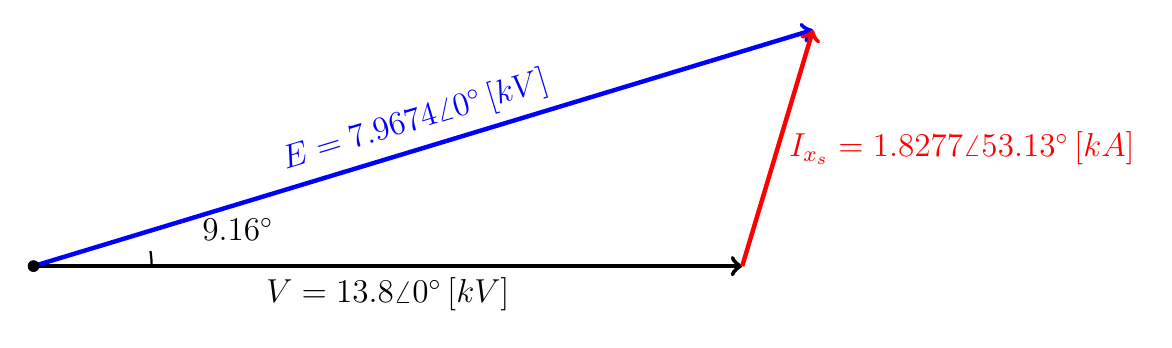
\begin{tikzpicture}

        % Definir los puntos
        \coordinate (O) at (0,0); % Origen
        \coordinate (V) at (9,0); % Punto V
        \coordinate (E) at (9.9,3); % Punto E con el ángulo
        
        % Dibujar las líneas más gruesas
        \draw[->, ultra thick, black] (O) -- (V) node[midway, below] {\large $V = 13.8 \angle 0^\circ \, \text{[kV]}$}; % Línea V
        \draw[->, ultra thick, blue] (O) -- (E) node[midway, above, sloped] {\large $E = 7.9674 \angle 0^\circ \, \text{[kV]}$}; % Línea E
        \draw[->, ultra thick, red] (V) -- (E) node[midway, right] {\large $I_{x_s} = 1.8277 \angle 53.13 ^\circ \, \text{[kA]}$}; % Línea corriente
        
        % Dibujar el ángulo con mejor ubicación
        \draw[thick] (1.5,0) arc[start angle=0,end angle=9.16,radius=1.2] node[above right, xshift=15] {\large $9.16^\circ$};
        
        % Añadir un punto para hacer el ángulo más visible
        \node at (O) [circle,fill,inner sep=1.5pt] {};
        
        \end{tikzpicture}
    \end{center}
    Como tenemos que $|\hat{E}| > |\hat{V}|$ luego podemos observar que el generador se encuentra sobreexcitado.
\end{solution}
%----------------------------
\end{questions}
\newpage
%%%%%%%%%%%%%%%%%%%%%%%%%%%


\end{document}